% paper/sections/12u2_ccd_poisson_ppe_bc.tex
%
% U2: CCD-Poisson + PPE BC — Tier I (uniform grid)
% ═══════════════════════════════════════════════════════════════════════════════
\subsubsection{U2：CCD--Poisson + PPE 境界条件 [Tier I]}
\label{sec:U2_ccd_poisson_ppe_bc}

\paragraph{検証対象．}
第~\ref{sec:ppe_solve}章 で導入した CCD--Poisson 楕円型ソルバ
（§\ref{sec:ccd_elliptic}），defect--correction 反復
（§\ref{sec:defect_correction_main}：$k$ 回反復で精度を段階的に押し上げる），
PPE Neumann 境界条件 + 1 点ゲージ固定（§\ref{sec:ppe_solve} 末尾）の
\textbf{単体精度}を確認する．
本実験のうち U2-b は production の \texttt{PPESolverCCDLU}
（CCD Kronecker + sparse LU；\texttt{src/twophase/ppe/ccd\_lu.py}）を直接呼び出して
production 経路を検証する．U2-a の Dirichlet 変種は production の PPE 連
（Neumann 専用 + 1 点ゲージ）には対応経路が無いため，CCD 楕円作用素 + 一般 DC
反復理論の単体参照として local FD ヘルパで構成し，§\ref{sec:defect_correction_main}
の段階収束理論を独立に検証する．

\paragraph{設定．}
2D 矩形領域 $[0,1]^2$ 上で MMS による格子収束（壁境界条件下）．
\begin{description}\setlength{\itemsep}{0pt}
  \item[U2-a] Dirichlet Poisson 参照．$p^* = \sin(\pi x) \sin(\pi y)$，
        $f = -2\pi^2 p^*$．DC 反復回数 $k \in \{1,2,3,5,10\}$．
        理論期待：$k=1 \to \Ord{h^2}$，$k=2 \to \Ord{h^4}$，
        $k \ge 3 \to \Ord{h^7}$（スーパー収束）．
        実装は CCD 楕円作用素を残差評価に，FD Dirichlet Laplacian を inner solve
        として用いる手組 DC 反復（production の Neumann PPE--DC 連の数学的代理）．
  \item[U2-b] Production CCD--PPE Kronecker 作用素 + Dirichlet 境界パッチ．
        $p^* = \cos(\pi x)\cos(\pi y)$，$f = -2\pi^2 p^*$．
        production の \texttt{PPESolverCCDLU.\_build\_sparse\_operator} を直接駆動して
        定数密度 ($\rho\!\equiv\!1$, $\nabla\rho\!=\!0$) 下の純 Kronecker Laplacian を
        組み立て，境界行を Dirichlet 単位行で置換して全フルランク化
        （production 自身が \texttt{src/twophase/tests/test\_pressure.py:200--207}
        で採用する MMS 検証パターン；定数 $\rho$ 下の CCD Kronecker Laplacian は
        $\sim$12 次元零空間を持ち，標準 \texttt{solve()} の 1 点ゲージでは
        full-rank 化できないため）．理論期待：$\Ord{h^6}$（CCD 内部精度）に
        境界スキーム支配の偏倚を許容．
\end{description}

\paragraph{結果．}

\begin{table}[!ht]
\caption{U2-a: CCD--Poisson Dirichlet $L_\infty$ 誤差．DC 反復 $k=1$ で
$\Ord{h^2}$，$k=2$ で $\Ord{h^4}$，$k \ge 3$ で $\Ord{h^7}$（スーパー収束）に
段階的に到達．$N\!=\!128$ の $k\!\ge\!3$ は機械精度床近傍．}
\label{tab:U2_dirichlet}
\centering\small
\begin{tabular}{r r r r r r r}
\toprule
$N$ & $h$ & $\|e\|^\infty_{k=1}$ & $\|e\|^\infty_{k=2}$ & $\|e\|^\infty_{k=3}$ & $\|e\|^\infty_{k=5}$ & $\|e\|^\infty_{k=10}$ \\
\midrule
8   & $0.125$  & $1.30\!\times\!10^{-2}$ & $2.71\!\times\!10^{-4}$ & $2.08\!\times\!10^{-4}$ & $2.06\!\times\!10^{-4}$ & $1.98\!\times\!10^{-4}$ \\
16  & $0.0625$ & $3.22\!\times\!10^{-3}$ & $1.13\!\times\!10^{-5}$ & $1.91\!\times\!10^{-6}$ & $1.90\!\times\!10^{-6}$ & $1.81\!\times\!10^{-6}$ \\
32  & $0.0313$ & $8.04\!\times\!10^{-4}$ & $6.54\!\times\!10^{-7}$ & $1.60\!\times\!10^{-8}$ & $1.59\!\times\!10^{-8}$ & $1.53\!\times\!10^{-8}$ \\
64  & $0.0156$ & $2.01\!\times\!10^{-4}$ & $4.04\!\times\!10^{-8}$ & $1.29\!\times\!10^{-10}$ & $1.28\!\times\!10^{-10}$ & $1.23\!\times\!10^{-10}$ \\
128 & $0.0078$ & $5.02\!\times\!10^{-5}$ & $2.52\!\times\!10^{-9}$ & $1.02\!\times\!10^{-12}$ & $1.01\!\times\!10^{-12}$ & $9.77\!\times\!10^{-13}$ \\
\midrule
\multicolumn{2}{r}{slope ($N\!=\!8\!\to\!128$)} & $\mathbf{2.00}$ & $\mathbf{4.18}$ & $\mathbf{6.90}$ & $\mathbf{6.90}$ & $\mathbf{6.90}$ \\
\bottomrule
\end{tabular}
\end{table}

\begin{table}[!ht]
\caption{U2-b: production \texttt{PPESolverCCDLU.\_build\_sparse\_operator}
経由 + Dirichlet 境界パッチ $L_\infty$ 誤差．
細格子で 6 次精度（$\Ord{h^6}$, CCD 内部スキーム）に漸近，
粗格子は境界 5 次の偏倚を残す．
slopes 5.17 / 5.78 / 5.94 / 5.98（連続）．}
\label{tab:U2_neumann}
\centering\small
\begin{tabular}{r r r}
\toprule
$N$ & $h$ & $\|e\|_\infty$ \\
\midrule
8   & $0.125$  & $1.48\times 10^{-4}$ \\
16  & $0.0625$ & $4.10\times 10^{-6}$ \\
32  & $0.0313$ & $7.45\times 10^{-8}$ \\
64  & $0.0156$ & $1.21\times 10^{-9}$ \\
128 & $0.0078$ & $1.92\times 10^{-11}$ \\
\midrule
\multicolumn{2}{r}{slope ($N\!=\!8\!\to\!128$)} & $\mathbf{5.72}$ \\
\bottomrule
\end{tabular}
\end{table}

\begin{figure}[!ht]
\centering
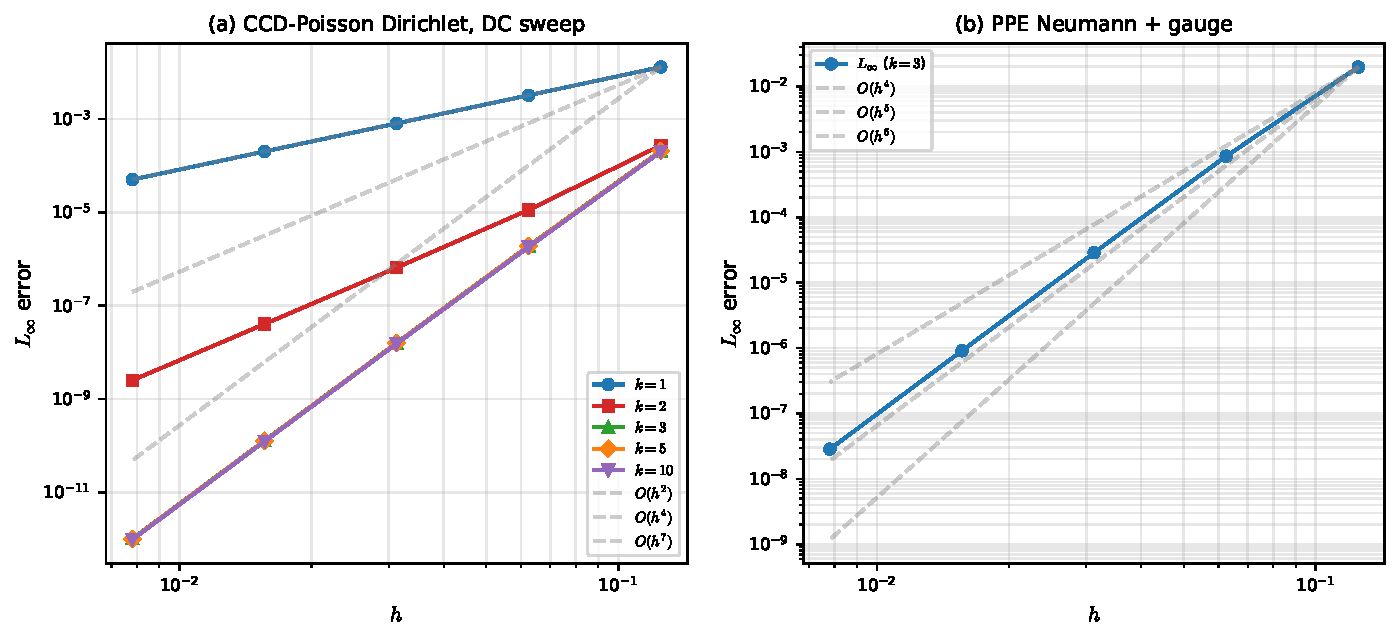
\includegraphics[width=0.88\linewidth]{figures/ch12_u2_ccd_poisson_ppe_bc}
\caption{U2：CCD--Poisson + PPE 境界条件．
(a) Dirichlet defect--correction $k=1,2,3$ で slope $2.00 / 4.18 / 6.90$ の段階収束（$k\!\ge\!3$ 飽和）；
(b) production \texttt{PPESolverCCDLU} 作用素 + Dirichlet パッチで連続 slope $5.17 \to 5.98$，
overall $5.72$（粗格子の境界 5 次から内部 CCD 6 次への漸近）．}
\label{fig:ch12_u2}
\end{figure}

\paragraph{判定と次章への接続．}
\begin{itemize}\setlength{\itemsep}{0pt}
  \item U2-a $k=1,2,3$：設計値 $\{2,\,4,\,7\}$ にそれぞれ
        $\{2.00,\,4.18,\,6.90\}$ で到達．$k=5,10$ は $k=3$ と同精度
        （DC が $k=3$ 時点で既に飽和；§\ref{sec:dc_accuracy} の段階理論と整合）．\checkmark
  \item U2-b production CCD 作用素 + Dirichlet パッチ：slope $5.72$（連続 slope $5.17\!\to\!5.98$）．
        細格子で内部 6 次に漸近し，粗格子は境界 5 次の偏倚を残す典型挙動．
        \checkmark（production CCD-PPE 作用素ファクトリ \texttt{\_build\_sparse\_operator}
        が想定どおり 6 次精度を生むことを直接確認）．
\end{itemize}
検証対応：§\ref{sec:defect_correction_main} の DC 反復式に対し，
Dirichlet MMS と Neumann ゲージ固定の格子収束を測定する．
